% Options for packages loaded elsewhere
\PassOptionsToPackage{unicode}{hyperref}
\PassOptionsToPackage{hyphens}{url}
%
\documentclass[
]{article}
\usepackage{amsmath,amssymb}
\usepackage{iftex}
\ifPDFTeX
  \usepackage[T1]{fontenc}
  \usepackage[utf8]{inputenc}
  \usepackage{textcomp} % provide euro and other symbols
\else % if luatex or xetex
  \usepackage{unicode-math} % this also loads fontspec
  \defaultfontfeatures{Scale=MatchLowercase}
  \defaultfontfeatures[\rmfamily]{Ligatures=TeX,Scale=1}
\fi
\usepackage{lmodern}
\ifPDFTeX\else
  % xetex/luatex font selection
\fi
% Use upquote if available, for straight quotes in verbatim environments
\IfFileExists{upquote.sty}{\usepackage{upquote}}{}
\IfFileExists{microtype.sty}{% use microtype if available
  \usepackage[]{microtype}
  \UseMicrotypeSet[protrusion]{basicmath} % disable protrusion for tt fonts
}{}
\makeatletter
\@ifundefined{KOMAClassName}{% if non-KOMA class
  \IfFileExists{parskip.sty}{%
    \usepackage{parskip}
  }{% else
    \setlength{\parindent}{0pt}
    \setlength{\parskip}{6pt plus 2pt minus 1pt}}
}{% if KOMA class
  \KOMAoptions{parskip=half}}
\makeatother
\usepackage{xcolor}
\usepackage[margin=1in]{geometry}
\usepackage{color}
\usepackage{fancyvrb}
\newcommand{\VerbBar}{|}
\newcommand{\VERB}{\Verb[commandchars=\\\{\}]}
\DefineVerbatimEnvironment{Highlighting}{Verbatim}{commandchars=\\\{\}}
% Add ',fontsize=\small' for more characters per line
\usepackage{framed}
\definecolor{shadecolor}{RGB}{248,248,248}
\newenvironment{Shaded}{\begin{snugshade}}{\end{snugshade}}
\newcommand{\AlertTok}[1]{\textcolor[rgb]{0.94,0.16,0.16}{#1}}
\newcommand{\AnnotationTok}[1]{\textcolor[rgb]{0.56,0.35,0.01}{\textbf{\textit{#1}}}}
\newcommand{\AttributeTok}[1]{\textcolor[rgb]{0.13,0.29,0.53}{#1}}
\newcommand{\BaseNTok}[1]{\textcolor[rgb]{0.00,0.00,0.81}{#1}}
\newcommand{\BuiltInTok}[1]{#1}
\newcommand{\CharTok}[1]{\textcolor[rgb]{0.31,0.60,0.02}{#1}}
\newcommand{\CommentTok}[1]{\textcolor[rgb]{0.56,0.35,0.01}{\textit{#1}}}
\newcommand{\CommentVarTok}[1]{\textcolor[rgb]{0.56,0.35,0.01}{\textbf{\textit{#1}}}}
\newcommand{\ConstantTok}[1]{\textcolor[rgb]{0.56,0.35,0.01}{#1}}
\newcommand{\ControlFlowTok}[1]{\textcolor[rgb]{0.13,0.29,0.53}{\textbf{#1}}}
\newcommand{\DataTypeTok}[1]{\textcolor[rgb]{0.13,0.29,0.53}{#1}}
\newcommand{\DecValTok}[1]{\textcolor[rgb]{0.00,0.00,0.81}{#1}}
\newcommand{\DocumentationTok}[1]{\textcolor[rgb]{0.56,0.35,0.01}{\textbf{\textit{#1}}}}
\newcommand{\ErrorTok}[1]{\textcolor[rgb]{0.64,0.00,0.00}{\textbf{#1}}}
\newcommand{\ExtensionTok}[1]{#1}
\newcommand{\FloatTok}[1]{\textcolor[rgb]{0.00,0.00,0.81}{#1}}
\newcommand{\FunctionTok}[1]{\textcolor[rgb]{0.13,0.29,0.53}{\textbf{#1}}}
\newcommand{\ImportTok}[1]{#1}
\newcommand{\InformationTok}[1]{\textcolor[rgb]{0.56,0.35,0.01}{\textbf{\textit{#1}}}}
\newcommand{\KeywordTok}[1]{\textcolor[rgb]{0.13,0.29,0.53}{\textbf{#1}}}
\newcommand{\NormalTok}[1]{#1}
\newcommand{\OperatorTok}[1]{\textcolor[rgb]{0.81,0.36,0.00}{\textbf{#1}}}
\newcommand{\OtherTok}[1]{\textcolor[rgb]{0.56,0.35,0.01}{#1}}
\newcommand{\PreprocessorTok}[1]{\textcolor[rgb]{0.56,0.35,0.01}{\textit{#1}}}
\newcommand{\RegionMarkerTok}[1]{#1}
\newcommand{\SpecialCharTok}[1]{\textcolor[rgb]{0.81,0.36,0.00}{\textbf{#1}}}
\newcommand{\SpecialStringTok}[1]{\textcolor[rgb]{0.31,0.60,0.02}{#1}}
\newcommand{\StringTok}[1]{\textcolor[rgb]{0.31,0.60,0.02}{#1}}
\newcommand{\VariableTok}[1]{\textcolor[rgb]{0.00,0.00,0.00}{#1}}
\newcommand{\VerbatimStringTok}[1]{\textcolor[rgb]{0.31,0.60,0.02}{#1}}
\newcommand{\WarningTok}[1]{\textcolor[rgb]{0.56,0.35,0.01}{\textbf{\textit{#1}}}}
\usepackage{graphicx}
\makeatletter
\def\maxwidth{\ifdim\Gin@nat@width>\linewidth\linewidth\else\Gin@nat@width\fi}
\def\maxheight{\ifdim\Gin@nat@height>\textheight\textheight\else\Gin@nat@height\fi}
\makeatother
% Scale images if necessary, so that they will not overflow the page
% margins by default, and it is still possible to overwrite the defaults
% using explicit options in \includegraphics[width, height, ...]{}
\setkeys{Gin}{width=\maxwidth,height=\maxheight,keepaspectratio}
% Set default figure placement to htbp
\makeatletter
\def\fps@figure{htbp}
\makeatother
\setlength{\emergencystretch}{3em} % prevent overfull lines
\providecommand{\tightlist}{%
  \setlength{\itemsep}{0pt}\setlength{\parskip}{0pt}}
\setcounter{secnumdepth}{-\maxdimen} % remove section numbering
\ifLuaTeX
  \usepackage{selnolig}  % disable illegal ligatures
\fi
\IfFileExists{bookmark.sty}{\usepackage{bookmark}}{\usepackage{hyperref}}
\IfFileExists{xurl.sty}{\usepackage{xurl}}{} % add URL line breaks if available
\urlstyle{same}
\hypersetup{
  pdftitle={Analysis},
  hidelinks,
  pdfcreator={LaTeX via pandoc}}

\title{Analysis}
\author{}
\date{\vspace{-2.5em}2024-01-04}

\begin{document}
\maketitle

About this site

\begin{verbatim}
## -- Attaching core tidyverse packages ------------------------ tidyverse 2.0.0 --
## v forcats   1.0.0     v stringr   1.5.1
## v lubridate 1.9.3     v tibble    3.2.1
## v purrr     1.0.2     v tidyr     1.3.0
## v readr     2.1.4     
## -- Conflicts ------------------------------------------ tidyverse_conflicts() --
## x dplyr::filter() masks stats::filter()
## x dplyr::lag()    masks stats::lag()
## i Use the conflicted package (<http://conflicted.r-lib.org/>) to force all conflicts to become errors
## 
## Attaching package: 'gridExtra'
## 
## 
## The following object is masked from 'package:dplyr':
## 
##     combine
\end{verbatim}

\begin{Shaded}
\begin{Highlighting}[]
\CommentTok{\# The statistics of universities located in Ankara in terms of being the first choice for  students}
\NormalTok{plot\_1 }\OtherTok{\textless{}{-}} \FunctionTok{ggplot}\NormalTok{(our\_data, }\FunctionTok{aes}\NormalTok{(}\AttributeTok{x =}\NormalTok{ Year, }\AttributeTok{y =}\NormalTok{ choice\_1st)) }\SpecialCharTok{+}
  \FunctionTok{geom\_col}\NormalTok{(}\AttributeTok{fill=}\StringTok{"pink"}\NormalTok{)}\SpecialCharTok{+}
  \FunctionTok{labs}\NormalTok{(}\AttributeTok{x =} \StringTok{"Year"}\NormalTok{,}\AttributeTok{y =} \StringTok{"The Number of choices in 1st place"}\NormalTok{)}\SpecialCharTok{+}
  \FunctionTok{ggtitle}\NormalTok{(}\StringTok{"The statistics of universities located in Ankara in terms of being the first choice for students"}\NormalTok{) }\SpecialCharTok{+}
  \FunctionTok{theme\_minimal}\NormalTok{() }\SpecialCharTok{+}
  \FunctionTok{theme}\NormalTok{(}\AttributeTok{axis.title =} \FunctionTok{element\_text}\NormalTok{(}\AttributeTok{color =} \StringTok{"purple"}\NormalTok{))}\SpecialCharTok{+}
  \FunctionTok{facet\_wrap}\NormalTok{(.}\SpecialCharTok{\textasciitilde{}}\NormalTok{ University)}
\FunctionTok{print}\NormalTok{(plot\_1)}
\end{Highlighting}
\end{Shaded}

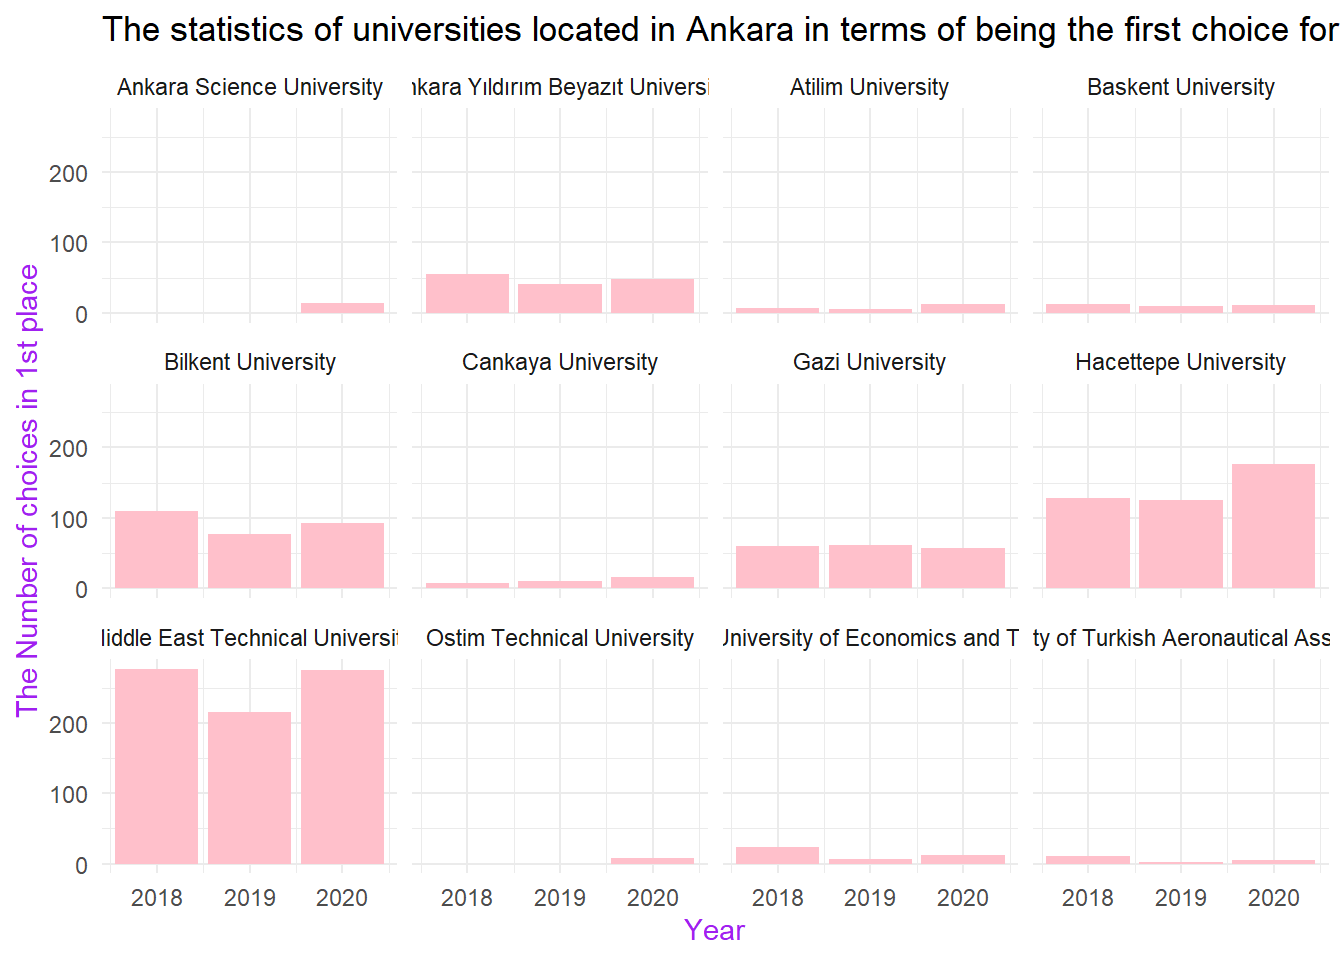
\includegraphics{presentationof_Emu430_files/figure-latex/unnamed-chunk-2-1.pdf}

Among the universities in Ankara, we thought that ODTÜ, Hacettepe, and
Bilkent University were most frequently chosen as the first preference,
and we have confirmed this by processing our data.

We can say that the first-choice selection for private universities such
as Ankara Bilim, Atılım, Çankaya, and Ostim Technical University has
increased over the years.We believe that this situation is created by
incentives provided by universities, such as internships, to their
students.

Additionally, among the State Universities, we observe that only
Hacettepe has an increasing trend in being the first choice.

\begin{Shaded}
\begin{Highlighting}[]
\NormalTok{avg\_first\_choices }\OtherTok{\textless{}{-}}\NormalTok{ our\_data }\SpecialCharTok{\%\textgreater{}\%} \FunctionTok{group\_by}\NormalTok{(University) }\SpecialCharTok{\%\textgreater{}\%} 
  \FunctionTok{summarise}\NormalTok{(}\AttributeTok{avg\_1st\_choices =} \FunctionTok{mean}\NormalTok{(choice\_1st)) }\SpecialCharTok{\%\textgreater{}\%}
  \FunctionTok{arrange}\NormalTok{(}\FunctionTok{desc}\NormalTok{(avg\_1st\_choices))}
\FunctionTok{print}\NormalTok{(avg\_first\_choices)}
\end{Highlighting}
\end{Shaded}

\begin{verbatim}
## # A tibble: 12 x 2
##    University                                      avg_1st_choices
##    <chr>                                                     <dbl>
##  1 Middle East Technical University                         256.  
##  2 Hacettepe University                                     143.  
##  3 Bilkent University                                        93.3 
##  4 Gazi University                                           59.3 
##  5 Ankara Yıldırım Beyazıt University                        48   
##  6 Ankara Science University                                 14   
##  7 Tobb Etu University of Economics and Technology           14   
##  8 Cankaya University                                        11.3 
##  9 Baskent University                                        11   
## 10 Atilim University                                          8.33
## 11 Ostim Technical University                                 8   
## 12 University of Turkish Aeronautical Association             6.33
\end{verbatim}

Here, when the averages of the choices for ODTÜ, Hacettepe, and Bilkent
are taken, we can comment that these universities are the most preferred
ones. Considering the rankings, we believe this table is consistent.

\begin{Shaded}
\begin{Highlighting}[]
\CommentTok{\#| code{-}fold: true}
\CommentTok{\#| code{-}summary: "Show the code"}

\CommentTok{\# The statistics of universities located in Ankara in terms of being the placed in 1st choice for students}
\NormalTok{plot\_2 }\OtherTok{\textless{}{-}} \FunctionTok{ggplot}\NormalTok{(our\_data, }\FunctionTok{aes}\NormalTok{(}\AttributeTok{x =}\NormalTok{ Year, }\AttributeTok{y =}\NormalTok{ placed\_1st)) }\SpecialCharTok{+} 
  \FunctionTok{geom\_col}\NormalTok{(}\AttributeTok{fill=}\StringTok{"lightblue"}\NormalTok{) }\SpecialCharTok{+}
 \FunctionTok{labs}\NormalTok{(}\AttributeTok{x =} \StringTok{"Year"}\NormalTok{,}\AttributeTok{y =} \StringTok{"The Number of students placed in first choice"}\NormalTok{)}\SpecialCharTok{+}
  \FunctionTok{ggtitle}\NormalTok{(}\StringTok{"The statistics of universities located in Ankara in terms of being the placed in first choice for students"}\NormalTok{) }\SpecialCharTok{+}
  \FunctionTok{theme\_minimal}\NormalTok{() }\SpecialCharTok{+}
  \FunctionTok{theme}\NormalTok{(}\AttributeTok{axis.title =} \FunctionTok{element\_text}\NormalTok{(}\AttributeTok{color =} \StringTok{"blue"}\NormalTok{))}\SpecialCharTok{+}
  \FunctionTok{facet\_wrap}\NormalTok{(.}\SpecialCharTok{\textasciitilde{}}\NormalTok{ University)}

\FunctionTok{print}\NormalTok{(plot\_2)}
\end{Highlighting}
\end{Shaded}

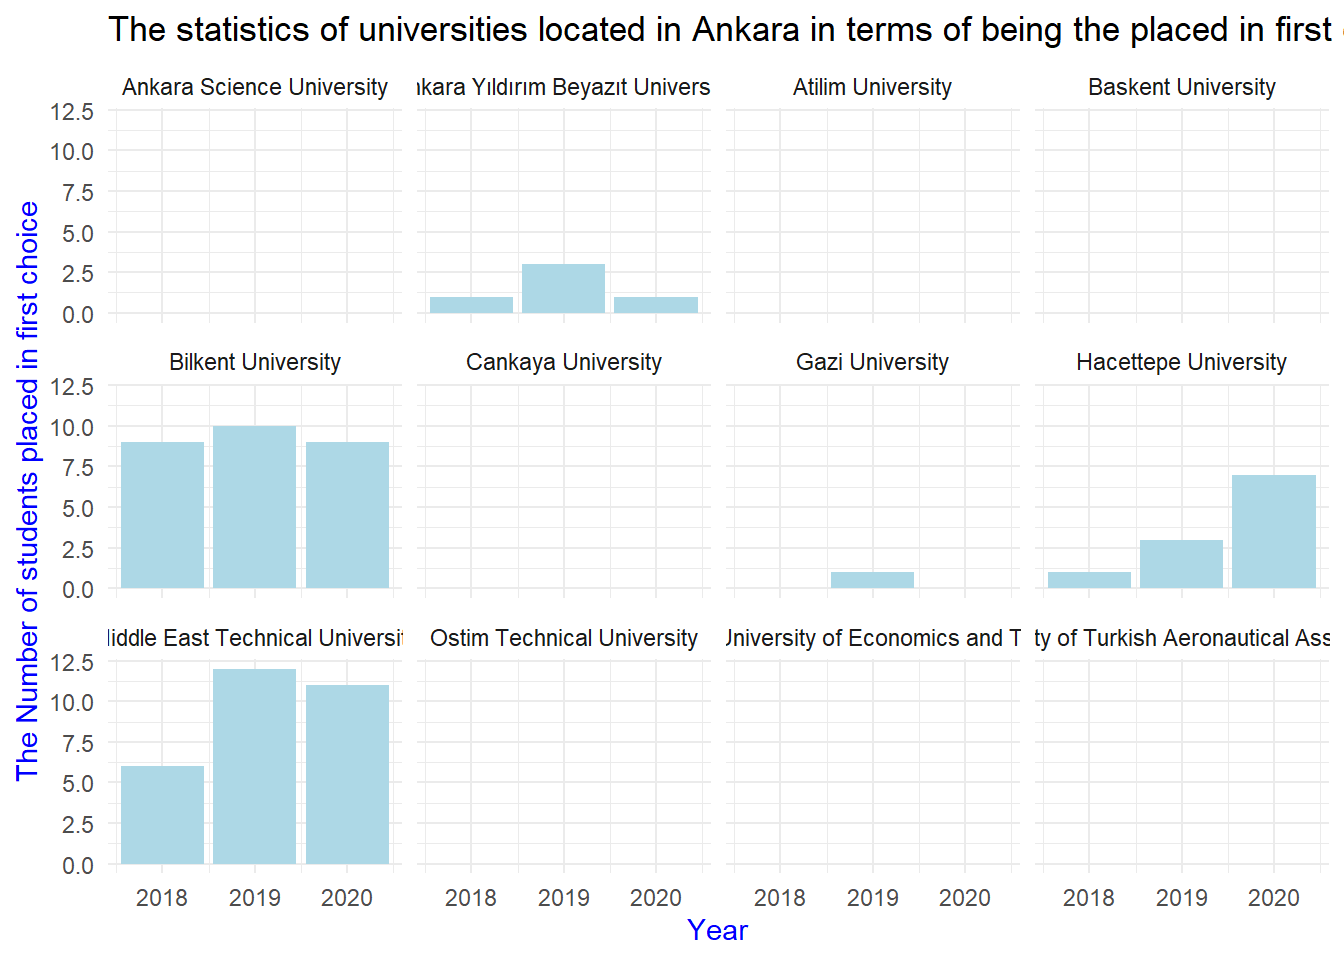
\includegraphics{presentationof_Emu430_files/figure-latex/unnamed-chunk-4-1.pdf}

This graph shows those who put the relevant university as their first
choice and got placed. Here, we observe that none of the private
universities showing an increase in the first graph demonstrated value.
This tells us that, despite being selected as the first choice, students
could not get placed in these universities.

In 2019, the placement situation for those who put these universities as
their first choice in Bilkent and ODTÜ was higher than Hacettepe, while
in 2020, we observe a decrease in these numbers. This explains the
increase in the number of students placed in Hacettepe in 2020. We think
that the students here shifted to Hacettepe.

\begin{Shaded}
\begin{Highlighting}[]
\CommentTok{\# Placement rate for students\textquotesingle{} first choices}


\NormalTok{placment\_rate\_data }\OtherTok{\textless{}{-}}\NormalTok{ our\_data }\SpecialCharTok{\%\textgreater{}\%} \FunctionTok{mutate}\NormalTok{(}\AttributeTok{placement\_rate =}\NormalTok{ placed\_1st}\SpecialCharTok{/}\NormalTok{choice\_1st) }\SpecialCharTok{\%\textgreater{}\%} \FunctionTok{select}\NormalTok{(Year, University, placement\_rate)}

\NormalTok{plot\_3 }\OtherTok{\textless{}{-}} \FunctionTok{ggplot}\NormalTok{(}\FunctionTok{na.omit}\NormalTok{(placment\_rate\_data), }\FunctionTok{aes}\NormalTok{(}\AttributeTok{x =} \FunctionTok{as.factor}\NormalTok{(Year), }\AttributeTok{y =}\NormalTok{ placement\_rate)) }\SpecialCharTok{+}
  \FunctionTok{geom\_col}\NormalTok{(}\AttributeTok{fill=}\StringTok{"lightgreen"}\NormalTok{) }\SpecialCharTok{+}
  \FunctionTok{labs}\NormalTok{(}\AttributeTok{x =} \StringTok{"Year"}\NormalTok{,}\AttributeTok{y =} \StringTok{"Placement Rate"}\NormalTok{)}\SpecialCharTok{+}
  \FunctionTok{ggtitle}\NormalTok{(}\StringTok{"Placement rate for students\textquotesingle{} first choices over year"}\NormalTok{) }\SpecialCharTok{+}
  \FunctionTok{theme\_minimal}\NormalTok{() }\SpecialCharTok{+}
  \FunctionTok{theme}\NormalTok{(}\AttributeTok{axis.title =} \FunctionTok{element\_text}\NormalTok{(}\AttributeTok{color =} \StringTok{"green"}\NormalTok{))}\SpecialCharTok{+}
  \FunctionTok{facet\_wrap}\NormalTok{(.}\SpecialCharTok{\textasciitilde{}}\NormalTok{ University)}

\FunctionTok{print}\NormalTok{(plot\_3)}
\end{Highlighting}
\end{Shaded}

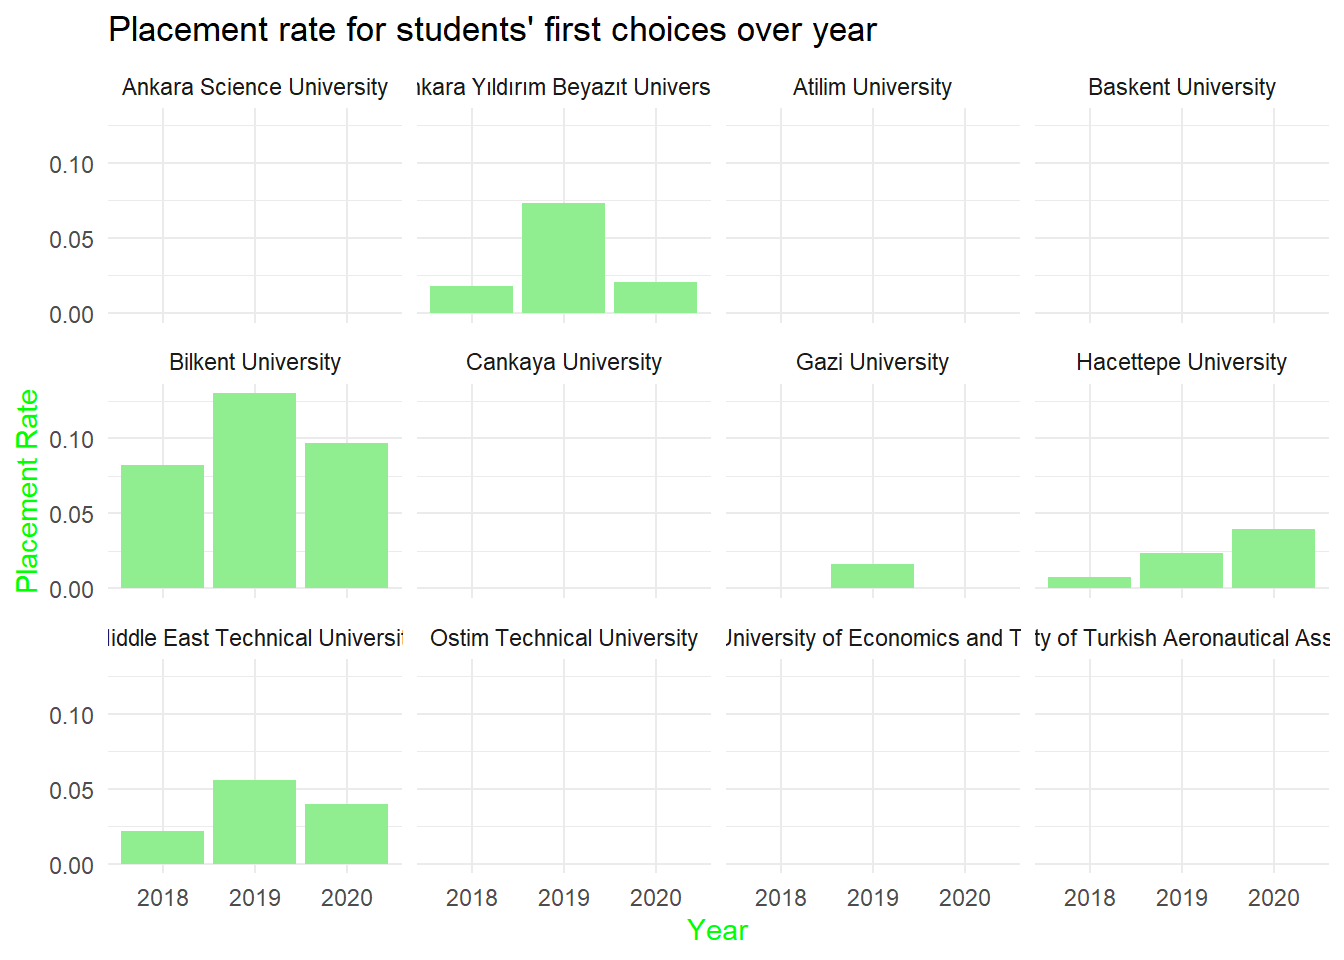
\includegraphics{presentationof_Emu430_files/figure-latex/unnamed-chunk-5-1.pdf}

This graph observes the ``writing as the first choice/placement'' ratio.
Higher-scored universities followed a more consistent path in the
preference stage.

\begin{Shaded}
\begin{Highlighting}[]
\CommentTok{\#| code{-}fold: true}
\CommentTok{\#| code{-}summary: "Show the code"}

\CommentTok{\# Hacettepe University Industrial Engineering data in 2018}

\NormalTok{hacettepe\_data1 }\OtherTok{\textless{}{-}}\NormalTok{ our\_data }\SpecialCharTok{\%\textgreater{}\%} \FunctionTok{filter}\NormalTok{(University }\SpecialCharTok{==} \StringTok{"Hacettepe University"}\NormalTok{,Year }\SpecialCharTok{==} \DecValTok{2018}\NormalTok{)}


\NormalTok{df\_long1 }\OtherTok{\textless{}{-}} \FunctionTok{pivot\_longer}\NormalTok{(hacettepe\_data1, }\AttributeTok{cols =} \FunctionTok{starts\_with}\NormalTok{(}\StringTok{"choice"}\NormalTok{),}
                        \AttributeTok{names\_to =} \StringTok{"Choice"}\NormalTok{, }\AttributeTok{values\_to =} \StringTok{"Value"}\NormalTok{)}

\NormalTok{plot\_4 }\OtherTok{\textless{}{-}} \FunctionTok{ggplot}\NormalTok{(df\_long1, }\FunctionTok{aes}\NormalTok{(}\AttributeTok{x=}\NormalTok{ Choice, }\AttributeTok{y =}\NormalTok{ Value))}\SpecialCharTok{+}
  \FunctionTok{geom\_col}\NormalTok{(}\AttributeTok{fill=}\StringTok{"pink"}\NormalTok{)}\SpecialCharTok{+}
  \FunctionTok{labs}\NormalTok{(}\AttributeTok{x =} \StringTok{"xnd chocie"}\NormalTok{,}\AttributeTok{y =} \StringTok{"The Number of choices "}\NormalTok{)}\SpecialCharTok{+}
  \FunctionTok{ggtitle}\NormalTok{(}\StringTok{"2018"}\NormalTok{) }\SpecialCharTok{+}
  \FunctionTok{theme\_minimal}\NormalTok{() }\SpecialCharTok{+}
  \FunctionTok{theme}\NormalTok{(}\AttributeTok{axis.title =} \FunctionTok{element\_text}\NormalTok{(}\AttributeTok{color =} \StringTok{"purple"}\NormalTok{))}\SpecialCharTok{+}
  \FunctionTok{theme}\NormalTok{(}\AttributeTok{axis.text.x =} \FunctionTok{element\_text}\NormalTok{(}\AttributeTok{angle =} \DecValTok{90}\NormalTok{, }\AttributeTok{hjust =} \DecValTok{1}\NormalTok{))}\SpecialCharTok{+}
  \FunctionTok{ylim}\NormalTok{(}\FunctionTok{c}\NormalTok{(}\DecValTok{0}\NormalTok{, }\DecValTok{220}\NormalTok{))}

\CommentTok{\# Hacettepe University Industrial Engineering data in 2019}

\NormalTok{hacettepe\_data2 }\OtherTok{\textless{}{-}}\NormalTok{ our\_data }\SpecialCharTok{\%\textgreater{}\%} \FunctionTok{filter}\NormalTok{(University }\SpecialCharTok{==} \StringTok{"Hacettepe University"}\NormalTok{,Year }\SpecialCharTok{==} \DecValTok{2019}\NormalTok{)}

\NormalTok{df\_long2 }\OtherTok{\textless{}{-}} \FunctionTok{pivot\_longer}\NormalTok{(hacettepe\_data2, }\AttributeTok{cols =} \FunctionTok{starts\_with}\NormalTok{(}\StringTok{"choice"}\NormalTok{),}
                        \AttributeTok{names\_to =} \StringTok{"Choice"}\NormalTok{, }\AttributeTok{values\_to =} \StringTok{"Value"}\NormalTok{)}

\NormalTok{plot\_5 }\OtherTok{\textless{}{-}} \FunctionTok{ggplot}\NormalTok{(df\_long2, }\FunctionTok{aes}\NormalTok{(}\AttributeTok{x=}\NormalTok{ Choice, }\AttributeTok{y =}\NormalTok{ Value))}\SpecialCharTok{+}
   \FunctionTok{geom\_col}\NormalTok{(}\AttributeTok{fill=}\StringTok{"lightblue"}\NormalTok{)}\SpecialCharTok{+}
  \FunctionTok{labs}\NormalTok{(}\AttributeTok{x =} \StringTok{"xnd chocie"}\NormalTok{,}\AttributeTok{y =} \StringTok{"The Number of choices"}\NormalTok{)}\SpecialCharTok{+}
  \FunctionTok{ggtitle}\NormalTok{(}\StringTok{"2019"}\NormalTok{) }\SpecialCharTok{+}
  \FunctionTok{theme\_minimal}\NormalTok{() }\SpecialCharTok{+}
  \FunctionTok{theme}\NormalTok{(}\AttributeTok{axis.title =} \FunctionTok{element\_text}\NormalTok{(}\AttributeTok{color =} \StringTok{"blue"}\NormalTok{))}\SpecialCharTok{+}
  \FunctionTok{theme}\NormalTok{(}\AttributeTok{axis.text.x =} \FunctionTok{element\_text}\NormalTok{(}\AttributeTok{angle =} \DecValTok{90}\NormalTok{, }\AttributeTok{hjust =} \DecValTok{1}\NormalTok{))}\SpecialCharTok{+}
  \FunctionTok{ylim}\NormalTok{(}\FunctionTok{c}\NormalTok{(}\DecValTok{0}\NormalTok{, }\DecValTok{220}\NormalTok{))}


\CommentTok{\# Hacettepe University Industrial Engineering data in 2020}
\NormalTok{hacettepe\_data3 }\OtherTok{\textless{}{-}}\NormalTok{ our\_data }\SpecialCharTok{\%\textgreater{}\%} \FunctionTok{filter}\NormalTok{(University }\SpecialCharTok{==} \StringTok{"Hacettepe University"}\NormalTok{,Year }\SpecialCharTok{==} \DecValTok{2020}\NormalTok{)}


\NormalTok{df\_long3 }\OtherTok{\textless{}{-}} \FunctionTok{pivot\_longer}\NormalTok{(hacettepe\_data3, }\AttributeTok{cols =} \FunctionTok{starts\_with}\NormalTok{(}\StringTok{"choice"}\NormalTok{),}
                         \AttributeTok{names\_to =} \StringTok{"Choice"}\NormalTok{, }\AttributeTok{values\_to =} \StringTok{"Value"}\NormalTok{)}

\NormalTok{plot\_6 }\OtherTok{\textless{}{-}} \FunctionTok{ggplot}\NormalTok{(df\_long3, }\FunctionTok{aes}\NormalTok{(}\AttributeTok{x=}\NormalTok{ Choice, }\AttributeTok{y =}\NormalTok{ Value)) }\SpecialCharTok{+} 
  \FunctionTok{geom\_col}\NormalTok{(}\AttributeTok{fill=}\StringTok{"lightgreen"}\NormalTok{)}\SpecialCharTok{+}
  \FunctionTok{labs}\NormalTok{(}\AttributeTok{x =} \StringTok{"xnd chocie"}\NormalTok{,}\AttributeTok{y =} \StringTok{"The Number of choices"}\NormalTok{)}\SpecialCharTok{+}
  \FunctionTok{ggtitle}\NormalTok{(}\StringTok{"2020"}\NormalTok{) }\SpecialCharTok{+}
  \FunctionTok{theme\_minimal}\NormalTok{() }\SpecialCharTok{+}
  \FunctionTok{theme}\NormalTok{(}\AttributeTok{axis.title =} \FunctionTok{element\_text}\NormalTok{(}\AttributeTok{color =} \StringTok{"green"}\NormalTok{))}\SpecialCharTok{+}
  \FunctionTok{theme}\NormalTok{(}\AttributeTok{axis.text.x =} \FunctionTok{element\_text}\NormalTok{(}\AttributeTok{angle =} \DecValTok{90}\NormalTok{, }\AttributeTok{hjust =} \DecValTok{1}\NormalTok{))}\SpecialCharTok{+}
  \FunctionTok{ylim}\NormalTok{(}\FunctionTok{c}\NormalTok{(}\DecValTok{0}\NormalTok{, }\DecValTok{220}\NormalTok{))}


\FunctionTok{print}\NormalTok{(}\FunctionTok{grid.arrange}\NormalTok{ (plot\_4, plot\_5, plot\_6, }\AttributeTok{ncol =} \DecValTok{3}\NormalTok{))}
\end{Highlighting}
\end{Shaded}

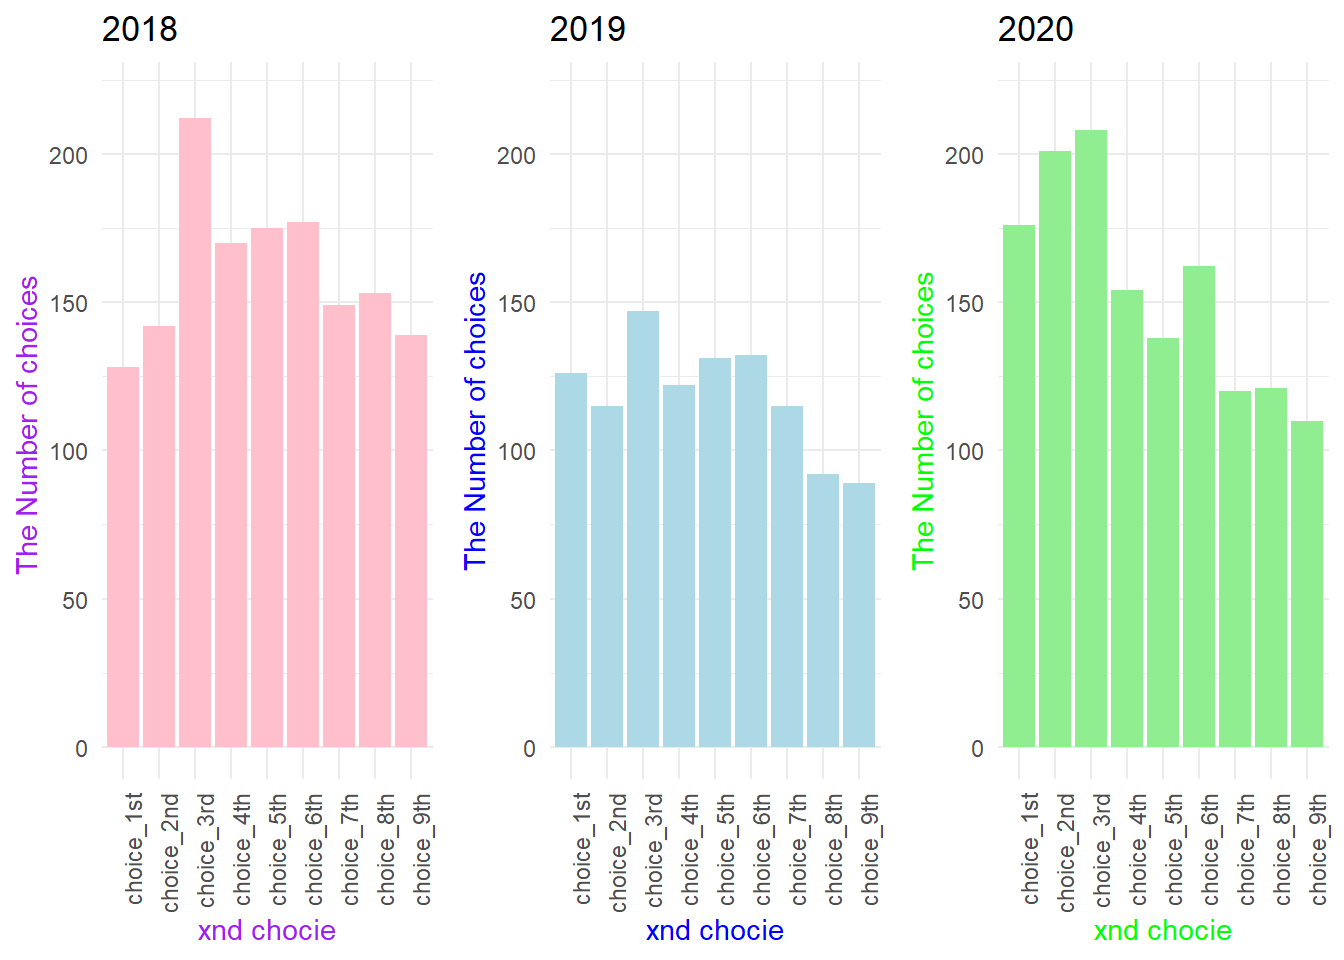
\includegraphics{presentationof_Emu430_files/figure-latex/unnamed-chunk-6-1.pdf}

\begin{verbatim}
## TableGrob (1 x 3) "arrange": 3 grobs
##   z     cells    name           grob
## 1 1 (1-1,1-1) arrange gtable[layout]
## 2 2 (1-1,2-2) arrange gtable[layout]
## 3 3 (1-1,3-3) arrange gtable[layout]
\end{verbatim}

This graph shows in which ranking Hacettepe was chosen within 3 years.
We can say that this graph supports our other graphs. We see that the
highest value is in the 3rd preference column. Similarly, we observe
that the first-choice selection situation increases over the years.

\end{document}
